\section{The Riemann-Roch theorem}
Equiped with sheaf cohomology, I will prove the Riemann-Roch theorem
using the methods we have learnt.
\begin{lnote}
  The rest of this paper will be concerned with algebraic curves. Thus,
  $X$ will always denote an irreducible, non-singular, complete algebraic
  curve over an algebraically closed field $k$. Such curves can be embedded
  in the projective space, see \cite{serre}. This allows us to assume that
  the field of rational functions $k(X)$ consists of functions $f/g$, where
  $f$ and $g$ are homogeneous polynomials over $k$ with $\deg f=\deg g$.
\end{lnote}

\subsection{Divisors and differentials}
Before tackling the Riemann-Roch theorem, I will quickly review two
constructions that we will need in the last two sections of this paper:
\emph{divisors} and \emph{differentials}. I use \cite{gathmann}
and \cite{serre} as my sources.

Like a sheaf, a divisor is an object that associates additional data to
an algebraic variety. Unlike sheaves, divisors contain \textbf{discrete}
data. More specifically, a divisor $D$ on $X$ associates an integer to
each point of $X$ and only finitely many of these integers are non-zero.
Then, we can represent the divisor as a formal linear combination
\[
  D=\sum_{P\in X}n_{P}P,
\]
where the integer $n_{P}$ is the value associated to the point $P$.
Now, two divisors can be added component by component so that divisors on
$X$ form an abelian group $\Div X$. Given a divisor $D$, I write $D(P)$
for the value $n_{P}$ associated to the point $P\in X$.
\begin{figure}[H]
  \centering
  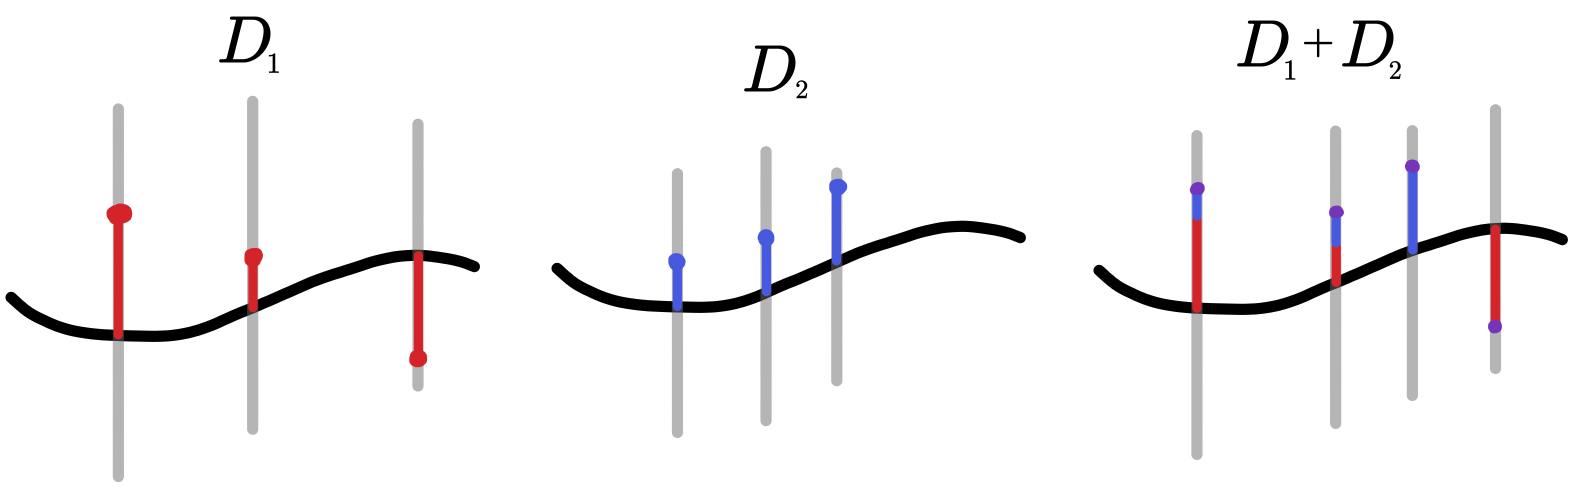
\includegraphics[width=\textwidth]{divisors}
  \caption{Visualising divisors and their sums}
\end{figure}
I will now define the \emph{degree} of a divisor and an order relation on
the group of divisors. The degree of a divisor $D$ is simply the integer
\[
  \deg(D) = \sum_{P\in X} D(P).
\]
Next, I say $D$ is \emph{effective} and write $D\geq 0$ if $D(P)\geq 0$
for all $P\in X$. Then, given two divisors $D, D^{\prime}$, I can define
$D\geq D^{\prime}$ if the divisor $D-D^{\prime}$ is effective.

Important types of divisors are the ones associated to a non-zero rational
function $f\in k(X)^{\times}$. For a point $P\in X$, the ring
$\mathscr{O}_{X,P}$ is a discrete valuation ring (DVR) with valuation
$\ord_{P}$. Then, the divisor of $f$ is defined as follows.
\[
  (f) = \sum_{P\in X}\ord_{P}(f)P.
\]
\begin{ex}
  Consider $X=\mathbb{P}^{1}$ and
  \[f(X_{0}, X_{1})=\frac{X_{1}-X_{0}}{X_{1}}\in k(X_{0}, X_{1}).\]
  Since $f(X_{0}, X_{1})$ is a unit in the the local rings
  $\mathscr{O}_{X,P}$ for $P\neq [1:0], [1:1]$, we have $\ord_{P}(f)=0$
  at those points $P$. The points $[1:0]$ and $[1:1]$ are contained in the
  affine piece $\mathbb{A}_{0}^{1}=\Set{[X_{0},X_{1}]\in\mathbb{P}^{1}\mid
    X_{0}\neq 0}$. The dehomogenised version of $f$ on $\mathbb{A}_{0}^{1}$ is
  given by $f(x)=\frac{x-1}x$. One can immediately see that
  $\ord_{P_{0}}(f)=-1$ for $P_{0}=[1:0]$ and $\ord_{P_{1}}(f)=1$ for
  $P_{1}=[1:1]$. Therefore,
  \[(f)=P_{1}-P_{0}.\]
\end{ex}
\begin{rem}
  The divisor of a rational function should be thought of as counting the
  orders of zeros and poles of the function.
\end{rem}
I will now prove a proposition that will be needed later.
\begin{prop}\label{prop:rational_deg_zero}
  Suppose $f\in k(X)^{\times}$. Then, $\deg\left((f)\right)=0$.
\end{prop}
\begin{proof}
  TODO.
\end{proof}
\begin{rem}
  Note that divisors of rational functions form a group since
  $(f)+(g)=(fg)$. Then, we can take the quotient of $\Div X$ by this group.
  The quotient is called the Picard group $\Pic X$ and its elements are
  called \textbf{divisor classes}. Thus, there is an equivalence relation on
  $\Div X$ such that
  \[
    D\sim D^{\prime}\iff \exists f\in k(X)^{\times},\ D^{\prime}=D+(f).
  \]
  Then, $D$ and $D^{\prime}$ are said to be \textbf{linearly equivalent}.
\end{rem}

Now, say I want to control the ``order of vanishing'' of a rational function
$f\in k(X)^{\times}$ at the points of the curve $X$. For example, if I want
$f$ to have a ``pole'' only at some point $P\in X$ with order at least $-2$,
I can express this requirement in the following way. Define a divisor
$D=-2P$. Then, I require that $(f)\geq D$. Conventionally, we would actually
set $D=2P$ and require that $(f)\geq -D$. This motivates us to define the
sheaf $\mathcal{L}(D)$ of such functions:
\[
  \left(\mathcal{L}(D)\right)(U)=\Set{f\in k(X)\mid
  \forall P\in U,\ \ord_{P}(f)\geq -D(P)}
\]
\begin{figure}[H]
  \centering
  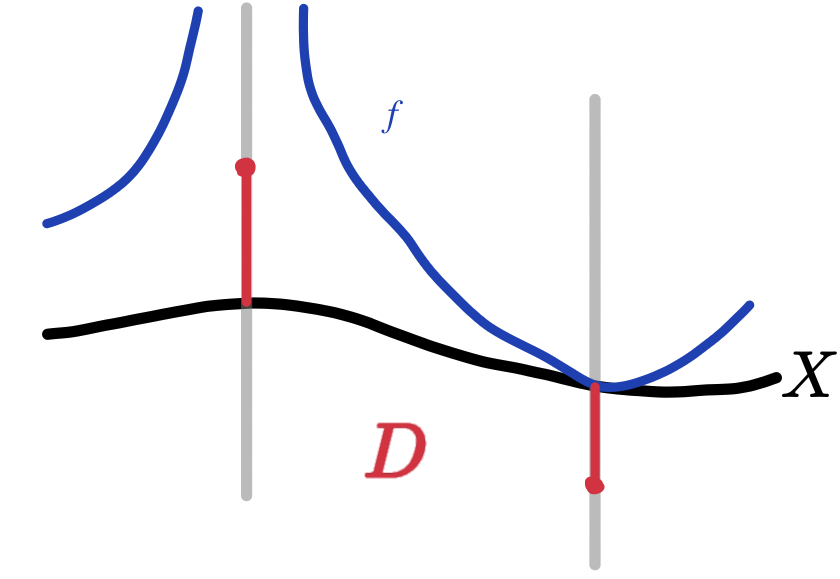
\includegraphics[width=.6\textwidth]{divisor_section}
  \caption{A section of the sheaf $\mathcal{L}(D)$}
\end{figure}
\begin{prop}
  The sheaves $\mathcal{L}(D)$ are quasi-coherent for every divisor $D$.
\end{prop}
\begin{proof}
  Firstly, $\mathcal{L}(D)$ is clearly a sheaf of $\mathscr{O}_{X}$-modules:
  If $f, g\in\mathcal{L}(D)(U)$, then it is clear that
  \[
    \forall P\in U,\ \ord_{P}(f+g)\geq -D(P).
  \]
  Moreover, if $h\in\mathscr{O}_{X}(U)$, then multiplying $f$ by $h$ only
  increases the order at all points, since $\ord_{P}(h)$ is never negative
  on $U$.

  Now, suppose $U\subseteq X$ is an affine open set and let $P\in U$ be a
  point where $D$ is non-zero. Then, take the open set
  $U_{P}^{\prime}\subseteq U$, which doesn't contain any of the other points
  where $D$ is non-zero. One can find a function $\phi_{P}\in k(X)$ in some
  neighbourhood $U_{P}\subseteq U_{P}^{\prime}$ of $P$ such that $(\phi_{P})=P$
  (by Lemma 7.5.6 in \cite{gathmann}). Now, multiplication by $\phi_{P}$
  defines an isomorphism $\mathcal{L}(D)(U_{P})\to \mathscr{O}_{U_{P}}$.
  Since quasi-coherence can be checked locally, this finishes the proof.
\end{proof}
The following proposition will also be useful later.
\begin{prop}\label{prop:global_sec_negative_divisor}
  If a divisor $D$ has negative degree, then $H^{0}(X,\mathcal{L}(D))=0$.
\end{prop}
\begin{proof}
  Suppose $f\in H^{0}(X,\mathcal{L}(D))$. Then, $(f)\geq -D$
  so that $\deg((f))\geq -\deg(D)$, but this implies $\deg(D)\geq 0$
  by Prop.~\ref{prop:rational_deg_zero}. This contradicts the assumption on
  $D$.
\end{proof}

I will now turn to discussing differentials. Recall the notion of the tangent
bundle, which is an integral concept in the local study of geometric spaces.
The typical definition of the tangent bundle given in calculus or
differential geometry does not translate directly to algebraic geometry.
Thus, we would need a more algebraic alternative. It turns out that it is
easier to give an algebraic definition of the \emph{cotangent bundle},
whose fibres are the dual spaces of the fibres of the tangent bundle. Now, I
will simply give the abstract definition of the cotangent bundle as a sheaf
of differentials. Giving geometric motivation for the definitions would take
us too far from the focus of the paper, and thus I leave it out. For a soft
exposition of differential forms in analysis, I recommend reading Terence
Tao's excellent article \cite{tao}.

\begin{defin}
  For a commutative algebra over the field $k$, the module of
  $k$-differentials of $F$ is the free $F$-module $\Omega(F)$ generated
  by the symbols $df$ for $f\in F$ with the following rules.
  \begin{itemize}
    \item $d(f+g)=df+dg$ for $f, g\in F$,
    \item $d(fg)=f\,dg+g\,df$ for $f, g\in F$,
    \item $da = 0$ for $a\in k$.
  \end{itemize}
\end{defin}
Note that this definition implies that the differential map $d:F\to\Omega(F)$
is $k$-linear: $d(af)=a\,df+f\,da=a\,df$ for $a\in k$. I will write
$\Omega$ for the module $\Omega\left(k(X)\right)$. Next, I can form a
quasi-coherent sheaf $\Omega_{X}$ by considering differentials of sections of
$\mathscr{O}_{X}$. Namely, by letting
$\Omega_{X}(U)=\Omega\left(\mathscr{O}_{X}(U)\right)$. One
immediately sees that this sheaf has the local structure one would expect:
$\Omega_{X,P}=\Omega\left(\mathscr{O}_{X,P}\right)$. Now, we can take
advantage of the DVR structure of the germs of the structure sheaf.
\begin{prop}
  Suppose $t$ is a local uniformiser of $\mathscr{O}_{X,P}$ at some
  point $P\in X$. Then, $\Omega$ is spanned by the differential $dt$.
\end{prop}
\begin{proof}
  Suppose $f\in k(X)$ is a rational function. Then it can be expressed as
  the quotient of two polynomials in $t$: $f=R(t)/S(t)$. One can calculate
  the differential corresponding to $f$ using the quotient rule:
  \[
    df = \frac{R^{\prime}(t)S(t)-R(t)S^{\prime}(t)}{S^{2}(t)}\,dt.
  \]
  As the generators $df$ of $\Omega$ are of the form $g\,dt$ for $g\in k(X)$,
  the statement follows.
\end{proof}
This proposition lets us to define the order of a differential
$\omega\in\Omega$ as follows. Write $\omega=f\,dt$ for $f\in k(X)$. Then,
\[
  \ord_{P}(\omega)=\ord_{P}(f).
\]
Now, we can define the divisor $(\omega)$ of $\omega$ in the same way as
the divisor of a rational function:
\[
  (\omega)=\sum_{P\in X}\ord_{P}(\omega)P.
\]
We can also define a module of differentials related to a divisor $D$
on $X$ in the same way as we defined the sheaf $\mathcal{L}(D)$:
\[
  \Omega(D)=\Set{\omega\in\Omega\mid \forall P\in X,\ \ord_{P}(\omega)
  \geq D(P)}.
\]
(in the modern literature one requires $\ord_{P}(\omega)\geq -D(P)$
to match the definition of $\mathcal{L}(D)$, but here I follow \cite{serre}
with the notation).

Lastly, I will define the \emph{residue} of a differential, which will be
the main ingredient in the proof of Serre duality in the next section.
\begin{defin}
  Let $\omega=f\,dt\in\Omega$, where $t$ is a local uniformiser of
  $\mathscr{O}_{X,P}$ for some point $P\in X$. Then, $f$ can be embedded
  in the ring $k((t))$ of formal series over $k$, where it has a series
  expansion in terms of $t$:
  \[
    f=\sum_{i\geq n}a_{i}t^{i},
  \]
  where $n\in\mathbb{Z}$ and $a_{i}\in k$. Then, the residue of $\omega$
  at $P$ is defined as $\res_{P}(\omega)=a_{-1}$.
\end{defin}
A priori, this definition depends on the local uniformiser $t$, and thus
I need to show that the definition is indeed independent of the choise
of a local uniformiser. I will only give a proof sketch, but a more detailed
proof can be found in \cite{serre}.
\begin{lemm}\label{lemm:res_quotient}
  For a non-zero function $f$, we have $\res_{P}(df/f)=\ord_{P}(f)$.
\end{lemm}
\begin{proof}
  If $t$ is a local uniformiser of $\mathscr{O}_{X,P}$, then $f$ can be
  written as $f=ut^{n}$, where $n=\ord_{P}(f)$. Then,
  \[
    df/f = \frac{t^{n}\,du + nut^{n-1}\,dt}{ut^{n}}=du/u+n\,dt/t.
  \]
  Thus, $\res_{P}(df/f)=\res_{t}(du/u)+n$, but since $u$ is a unit in
  $\mathscr{O}_{X,P}$, the residue $\res_{t}(du/u)$ is clearly zero.
\end{proof}
\begin{prop}
  Fix a point $P\in X$ and let $t$ and $r$ be two local uniformisers of
  $\mathscr{O}_{X,P}$. Denote by $\res_{t}$ and $\res_{r}$ the function
  $\res_{P}$ calculated using $t$ and $r$ respectively. Then,
  $\res_{t}(\omega)=\res_{r}(\omega)$ for all differentials $\omega\in\Omega$.
\end{prop}
\begin{proof}[Proof sketch]
  Suppose $f\in k(X)$ is a rational function with a series expansion
  \[
    f=\sum_{i\geq n}a_{i}t^{i},
  \]
  in $t$. Then, it is possible to construct a module of differentials, where
  \[
    df=\left(\sum_{i\geq n}ia_{i}t^{i-1}\right)\,dt.
  \]
  This is probably the most non-trivial statement of the proof, and the
  construction can be found in \cite{serre}. Now, we can write a
  differential $\omega$ in this module as
  \[
    \omega = \sum_{n\geq 0}a_{n}\,du/u^{n}+\omega_{0},
  \]
  where $\omega_{0}$ is a differential with $\ord_{P}(\omega_{0})\geq 0$.
  Then, $\res_{u}(\omega)=a_{1}$ and $\res_{t}(\omega)=
  \sum a_{n}\res_{t}(du/u^{n})$. Now, consentrate first on the term
  $a_{1}\res_{t}(du/u)$. I can apply Lemma~\ref{lemm:res_quotient}
  to get $\res_{t}(du/u)=\ord_{P}(u)=1$. Therefore,
  \[
    \res_{t}(\omega) = a_{1}+\sum_{n>0}\res_{t}(du/u^{n}).
  \]
  Hence, it is enough to show that $\res_{t}(du/u^{n})=0$ for $n>0$.

  In characteristic zero, we can write
  \[
    du/u^{n}=d\left(-\frac1{(n-1)u^{n-1}}\right).
  \]
  But this immediately implies that $\res_{t}(du/u^{n})=0$ since
  differentiating a series can never result in a term of the form
  $a_{-1}t^{-1}$. The proof for positive characteristic follows from the
  statement in zero characteristic and can be found in \cite{serre}.
\end{proof}
Now, I will prove the \emph{residue theorem}, which is used in the proof
of the Serre duality theorem.
\begin{thm}[Residue Theorem]\label{thm:residue_theorem}
  For every differential $\omega\in\Omega$, we have that
  \[
    \sum_{P\in X}\res_{P}(\omega)=0.
  \]
\end{thm}
First I prove the theorem for the case when $X=\mathbb{P}^{1}_{k}$.
\begin{lemm}
  The residue theorem holds for $X=\mathbb{P}^{1}_{k}$.
\end{lemm}
\begin{proof}
  Fix a differential $\omega=f\,dt$ on $X$. For convenience, I work with
  dehomogenised representation, and take $f$ to be a rational function
  in one variable $t$. This function has a partial fractions decomposition,
  which is a linear combination of terms of the form listed below. I will
  consider each type separately.
  \begin{description}[style=nextline]
    \item[Term of type $\omega=t^{n}\,dt$:] There are no poles at finite
          points, so the only pole could be at infinity. Changing to
          $u=1/t$, we have $dt=-u^{-2}\,du$ and
          \[\omega=(u^{-n})(-u^{-2}\,du)=\frac{du}{u^{n+2}}.\]
          Then, the residue clearly vanishes: $\res_{\infty}(\omega)=0$.
    \item[Term of type $\omega=\frac{dt}{t-a}$:] Clearly $\res_{a}(\omega)=1$,
          and there are no other poles at finite points. But there is also a
          pole at infinity. Again, changing to $u=1/t$, we get
          \begin{align*}
            f(u)&=\left(\frac{u}{1-au}\right)(-u^{-2}\,du)
            =-\frac1{u}\cdot\frac1{1-au}\,du \\
            &=-\frac1{u}\left(1+au+(au)^{2}+\cdots\right)\,du.
          \end{align*}
          Therefore, $\res_{a}(\omega)=-1$ and the residues of the two points
          cancel.
    \item[Term of type $\omega=\frac{dt}{(t-a)^{n}}$ for $n>1$:] Following
          a similar argument as above, one can check that in this case
          the residue is zero also at $a$ and $\infty$.
  \end{description}
\end{proof}
Let $X$ be a curve as before. The strategy now is to consider a non-constant
function $\phi\in k(X)$. Such a function gives a morphism
$\phi:X\to\mathbb{P}^{1}_{k}$, which induces an embedding
$k(\mathbb{P}^{1}_{k})\hookrightarrow k(X)$. I hope to use this embedding
to use the above lemma in the case of an arbitrary curve $X$.
Now, one can consider the trace map $\tr_{k(X)/k(\mathbb{P}^{1}_{k})}$ defined
as follows \cite{milne}. Multiplication by an element $\alpha\in k(X)$
defines a $k(\mathbb{P}^{1}_{k})$-linear map
$\alpha^{\ast}: E\to E: x\mapsto \alpha x$. Then, we simply define
$\tr_{k(X)/k(\mathbb{P}^{1}_{k})}(\alpha)$ to be the usual trace of this linear
transformation $\alpha^{\ast}$. Next I translate this definition to
differentials on $k(X)$. We can write any differential
$\omega\in\Omega(k(X))$ as $\omega=f\,d\phi$. Then, one can make the
following definition.
\[
  \tr:\Omega(k(X))\to \Omega(k(\mathbb{P}^{1}_{k}))
  :f\,d\phi\mapsto \left(\tr_{k(X)/k(\mathbb{P}^{1}_{k})}(f)\right)\,d\phi
\]
Finally, the residue formula is implied by the following lemma which
is proved in \cite{serre}.
\begin{lemm}
  For every point $P\in\mathbb{P}^{1}_{k}$, we have
  \[
    \sum_{Q\in\phi^{-1}(P)}\res_{Q}(\omega)=\res_{P}(\tr(\omega)).
  \]
\end{lemm}

\subsection{Proof of Riemann-Roch}
I am now able to state and prove an ``incomplete'' version of the
Riemann-Roch theorem, which I will make complete after proving Serre
duality.

% TODO: Give a proof that the cohomology groups are finite-dimensional.

\begin{thm}[Riemann-Roch, cohomology version]
  \label{thm:riemann_roch_cohomology}
  For every divisor $D$,
  \[
    h^{0}(X, \mathcal{L}(D))-h^{1}(X, \mathcal{L}(D))=\deg(D)+1-g,
  \]
  where $g=h^{1}(X, \mathscr{O}_{X})$.
\end{thm}
\begin{proof}
  One can use an induction argument, because any divisor $D$ can be
  obtained from the zero divisor by adding and subtracting points.
  Thus, I proceed by first proving the base case and then proving
  the induction step.

  \begin{description}[style=nextline]
    \item[base case$\big)$]
          Since $\mathcal{L}(0)=\mathscr{O}_{X}$ and $\deg(0)=0$,
          I need to verify that
          \[h^{0}(X, \mathscr{O}_{X})-h^{1}(X, \mathscr{O}_{X})=1-g.\]
          But note that the only globally defined regular functions
          on $X$ are constant and thus they form a one-dimensional vector
          space. Moreover, $h^{1}(X, \mathscr{O}_{X})=g$ by definition
          so that the equality holds.
    \item[induction step$\big)$]
          In the induction step I want to relate the 0th and the 1st
          cohomology groups of $\mathcal{L}(D)$ to the 0th and
          1st cohomology groups of $\mathcal{L}(D+P)$, where
          $P$ is some point. To do this, first note that
          $\mathcal{L}(D)$ is a subsheaf of $\mathcal{L}(D+P)$, since
          the orders of the sections of $\mathcal{L}(D+P)$ at $P$ are
          allowed to be smaller than the orders of the sections of
          $\mathcal{L}(D)$ at $P$. Thus, there is an exact sequence
          \[
          \begin{tikzcd}
            0\arrow{r} & \mathcal{L}(D)\arrow{r} & \mathcal{L}(D+P)\arrow{r}
            & Q\arrow{r} & 0,
          \end{tikzcd}
          \]
          where $Q$ is the quotient sheaf. The stalks of $Q$ are clearly
          zero away from $P$. The stalk at $P$ consists of zero and
          elements of the form $u/t^{n+1}$, where $t$ is the local
          uniformiser of $\mathscr{O}_{X,P}$, $u$ is a unit in
          $\mathcal{O}_{X,P}$, and $n$ is the order of $P$ in $D$.
          As $\mathcal{O}_{X,P}/(t)=k$, we can write $u=vt+r$,
          where $v\in\mathcal{O}_{X,P}$ and $r\in k$.
          Then,
          \[\frac{u}{t^{n+1}}=\frac{v}{t^n}+\frac{r}{t^{n+1}}.\]
          Since $v/t^n$ is an element of $\mathcal{L}(D)_{P}$, we conclude
          that every element of $\mathcal{L}(D+P)_{P}$ is equivalent to
          an element $r/t^{n+1}$ modulo $\mathcal{L}(D)_{P}$ for some
          $r\in k$. Therefore, $Q_{P}\cong k$ and $Q$ is the skyscraper sheaf
          $k_{P}$.

          Now we apply our cohomology machinery on the SES
          \[
          \begin{tikzcd}
            0\arrow{r} & \mathcal{L}(D)\arrow{r} & \mathcal{L}(D+P)\arrow{r}
            & k_{P}\arrow{r} & 0
          \end{tikzcd}
          \]
          to get the following exact sequence (using
          Prop.~\ref{prop:sky_cohom}).
          \[
          \begin{tikzcd}
            0\arrow{r} & H^{0}(X, \mathcal{L}(D))\arrow{r}
            & H^{0}(X, \mathcal{L}(D+P))\arrow{r}
            & H^{0}(X, k_{P}) \\
            \arrow{r} & H^{1}(X, \mathcal{L}(D))\arrow{r}
            & H^{1}(X, \mathcal{L}(D+P))\arrow{r} & 0.
          \end{tikzcd}
          \]
          Now, this exact sequence of vector spaces implies the following
          equality.
          \[
          h^{0}(X,\mathcal{L}(D))-h^{0}(X, \mathcal{L}(D+P))
          +1-h^{1}(X,\mathcal{L}(D))+h^{1}(X,\mathcal{L}(D+P)) = 0.
          \]
          Therefore,
          \begin{align*}
            h^{0}(X,\mathcal{L}(D+P))&-h^{1}(X,\mathcal{L}(D+P))
            =\left(h^{0}(X,\mathcal{L}(D))-h^{1}(X,\mathcal{L}(D+P))\right)
              +1 \\
            =&\deg(D)+1-g+1\quad\text{(by induction hypothesis)} \\
            =&\deg(D+P)+1-g.
          \end{align*}
          This is exactly the induction step we wanted to prove.
          We also need to prove
          \[
            h^{0}(X,\mathcal{L}(D-P))-h^{1}(X,\mathcal{L}(D-P))
            =\deg(D-P)+1-g,
          \]
          but we can run the same argument starting with the SES
          \[
          \begin{tikzcd}
            0\arrow{r} & \mathcal{L}(D-P)\arrow{r} & \mathcal{L}(D)\arrow{r}
            & k_{P}\arrow{r} & 0.
          \end{tikzcd}
          \]
  \end{description}
\end{proof}

This form of the theorem is not the most useful one for applications,
because computing $h^{1}(X,\mathcal{L}(D))$ is not easy. Luckily, the Serre
Duality theorem --- which I will prove in the next section --- gives the
following equality of dimensions:
\[h^{1}(X,\mathcal{L}(D))=h^{0}(X,\mathcal{L}(K_{X}-D))\]
Now, this equality lets us write the ``complete'' form of the Riemann-Roch
theorem.
\begin{thm}[Riemann-Roch]\label{thm:riemann_roch}
  For every divisor $D$,
  \[
    h^{0}(X, \mathcal{L}(D))-h^{0}(X, \mathcal{L}(K_{X}-D))=\deg(D)+1-g,
  \]
  where $g=h^{1}(X, \mathcal{O}_{X})$.
\end{thm}

%\subsection{Applications to the classification of curves}
%Before proving the Serre duality theorem, I want to take some time to
%look at applications of the Riemann-Roch theorem.
\subsection{An application to the classification of curves}
Before proving the Serre duality theorem, I want to take some time to
look at an application of the Riemann-Roch theorem using \cite{hartshorne}
as my source. A major project in algebraic geometry is to give a
classification of different algebraic varieties. The Riemann-Roch theorem
helps us prove statements about varieties based solely on topological data,
namely the genus of the curve. First, I give a formula for the degree
of the canonical divisor on a curve.
\begin{lemm}
  The degree of the canonical divisor $K_{X}$ is $2g-2$, where $g$ is the
  genus of $X$.
\end{lemm}
\begin{proof}
  Set $D=K_{X}$ so that the Riemann-Roch theorem yields
  \begin{align*}
    h^{0}(X,\mathcal{L}(K_{X}))-h^{0}(X,\mathscr{O}_{X})&=\deg(D)+1-g \\
    h^{1}(X,\mathscr{O}_{X})-1&=\deg(D)+1-g \\
    2g-2&=\deg(D),
  \end{align*}
  where $h^{0}(X,\mathcal{L}(K_{X}))=h^{1}(X,\mathscr{O}_{X})$ is given
  by the Serre duality theorem.
\end{proof}
Now I can give a classification of curves of genus 0.
\begin{thm}
  Any curve $X$ of genus 0 is isomorphic to $\mathbb{P}^{1}_{k}$.
\end{thm}
\begin{proof}
  Fix two point $P,Q\in X$ and consider the divisor $D=P-Q$. The Riemann-Roch
  theorem implies
  \[
    h^{0}(X,\mathcal{L}(D))-h^{0}(X,\mathcal{L}(K_{X}-D))
    =\deg(D)+1=1.
  \]
  Note that $\deg(K_{X}-D)=-2-0=-2<0$ so $h^{0}(X,\mathcal{L}(K_{X}-D))=0$
  by Prop.~\ref{prop:global_sec_negative_divisor}. Therefore, the space
  $H^{0}(X,\mathcal{L}(D))$ is non-empty. Thus, let
  $f\in H^{0}(X,\mathcal{L}(D))$.
\end{proof}
